\documentclass[12pt,a4paper,oneside]{book}

		% --------------------------------- 페이지 스타일 지정
		\usepackage{geometry}
		\geometry{top=1.4in}
		\geometry{bottom=1.4in}
		\geometry{left=1.2in}
		\geometry{right=1.2in}
		\geometry{headheight=0.4in}
		\geometry{headsep=0.1in}
		\geometry{footskip=0.3in}
	%	\geometry{showframe}
	
		\newgeometry{ 	top=8em, bottom=8em,
						left=8em, right=8em, 
						headheight=2em, headsep=2em}


		%	===================================================================
		%	package
		%	===================================================================
%			\usepackage[hangul]{kotex}				% 한글 사용
			\usepackage{kotex}						% 한글 사용
			\usepackage[unicode]{hyperref}			% 한굴 하이퍼링크 사용
			\usepackage{amssymb,amsfonts,amsmath}	% 수학 수식 사용

			\usepackage{scrextend}					% 
		
			\usepackage{enumerate}			%
			\usepackage{enumitem}			%
			\usepackage{tablists}			%	수학문제의 보기 등을 표현하는데 사용
										%	tabenum


		% ------------------------------ table 
			\usepackage{longtable}			%
			\usepackage{tabularx}			%

			\usepackage{setspace}			%
			\usepackage{booktabs}			% table
			\usepackage{color}				%
			\usepackage{multirow}			%
			\usepackage{boxedminipage}		% 미니 페이지
			\usepackage[pdftex]{graphicx}	% 그림 사용
			\usepackage[final]{pdfpages}	% pdf 사용
			\usepackage{framed}			% pdf 사용
			
			\usepackage{fix-cm}	
			\usepackage[english]{babel}
	
			\usepackage{tikz}%
			\usetikzlibrary{arrows,positioning,shapes}
			%\usetikzlibrary{positioning}
			

		% --------------------------------- page
			\usepackage{afterpage}		% 다음페이지가 나온면 어떻게 하라는 명령 정의 패키지


			\usepackage{blindtext}
	
		% --------------------------------- font 사용
			\usepackage{pifont}				%
			\usepackage{textcomp}
			\usepackage{gensymb}
			\usepackage{marvosym}






		% --------------------------------- 페이지 스타일 지정

		\usepackage[Bjornstrup]{fncychap}

		\usepackage{fancyhdr}
		\pagestyle{fancy}
		\fancyhead{} % clear all fields
		\fancyhead[LO]{\footnotesize \leftmark}
		\fancyhead[RE]{\footnotesize \leftmark}
		\fancyfoot{} % clear all fields
		\fancyfoot[LE,RO]{\large \thepage}
		%\fancyfoot[CO,CE]{\empty}
		\renewcommand{\headrulewidth}{1.0pt}
		\renewcommand{\footrulewidth}{0.4pt}
	
	
	
		% --------------------------------- 	section 스타일 지정
	
		\usepackage{titlesec}
		
		\titleformat*{\section}		{\large\bfseries}
		\titleformat*{\subsection}		{\normalsize\bfseries}
		\titleformat*{\subsubsection}	{\normalsize\bfseries}
		\titleformat*{\paragraph}		{\normalsize\bfseries}
		\titleformat*{\subparagraph}	{\normalsize\bfseries}
	
		\renewcommand{\thesection}		{\arabic{section}.}
		\renewcommand{\thesubsection}	{\thesection\arabic{subsection}.}
		\renewcommand{\thesubsubsection}{\thesubsection\arabic{subsubsection}}
		
		\titlespacing*{\section} 		{0pt}{1.0em}{1.0em}
		\titlespacing*{\subsection}	  	{0ex}{1.0em}{1.0em}
		\titlespacing*{\subsubsection}	{0ex}{1.0em}{1.0em}
		\titlespacing*{\paragraph}		{0ex}{1.0em}{1.0em}
		\titlespacing*{\subparagraph}	{0ex}{1.0em}{1.0em}
	
	%	\titlespacing*{\section} 		{0pt}{0.0\baselineskip}{0.0\baselineskip}
	%	\titlespacing*{\subsection}	  	{0ex}{0.0\baselineskip}{0.0\baselineskip}
	%	\titlespacing*{\subsubsection}	{6ex}{0.0\baselineskip}{0.0\baselineskip}
	%	\titlespacing*{\paragraph}		{6pt}{0.0\baselineskip}{0.0\baselineskip}
	

		% --------------------------------- recommend		섹션별 페이지 상단 여백
		\newcommand{\SectionMargin}{\newpage  \null \vskip 2cm}
		\newcommand{\SubSectionMargin}{\newpage  \null \vskip 2cm}
		\newcommand{\SubSubSectionMargin}{\newpage  \null \vskip 2cm}


	
		% ----------------------------- 장의 목차
		\usepackage{minitoc}
		\setcounter{minitocdepth}{1}    	% Show until subsubsections in minitoc
		\setlength{\mtcindent}{12pt} 		% default 24pt
	
	
		% --------------------------------- 	문서 기본 사항 설정
		\setcounter{secnumdepth}{3} 		% 문단 번호 깊이
		\setcounter{tocdepth}{3} 			% 문단 번호 깊이
		\setlength{\parindent}{0cm} 		% 문서 들여 쓰기를 하지 않는다.
		
		
		% --------------------------------- 	줄간격 설정
		\doublespace
%		\onehalfspace
%		\singlespace
		
		
% 	============================================================================== List global setting
%		\setlist{itemsep=1.0em}
	
% 	============================================================================== enumi setting

%		\renewcommand{\labelenumi}{\arabic{enumi}.} 
%		\renewcommand{\labelenumii}{\arabic{enumi}.\arabic{enumii}}
%		\renewcommand{\labelenumii}{(\arabic{enumii})}
%		\renewcommand{\labelenumiii}{\arabic{enumiii})}


	%	-------------------------------------------------------------------------------
	%		Vertical and Horizontal spacing
	%	-------------------------------------------------------------------------------
		\setlist[enumerate,1]	{ leftmargin=8.0em, rightmargin=0.0em, labelwidth=0.0em, labelsep=0.0em }
		\setlist[enumerate,2]	{ leftmargin=8.0em, rightmargin=0.0em, labelwidth=0.0em, labelsep=0.0em }
		\setlist[enumerate,3]	{ leftmargin=8.0em, rightmargin=0.0em, labelwidth=0.0em, labelsep=0.0em }
		\setlist[enumerate]	{ itemsep=1.0em, leftmargin=6.0ex, rightmargin=0.0em, labelwidth=0.0em, labelsep=4.0ex }


	%	-------------------------------------------------------------------------------
	%		Label
	%	-------------------------------------------------------------------------------
%		\setlist[enumerate,1]{ label=\arabic*., ref=\arabic* }
%		\setlist[enumerate,1]{ label=\emph{\arabic*.}, ref=\emph{\arabic*} }
%		\setlist[enumerate,1]{ label=\textbf{\arabic*.}, ref=\textbf{\arabic*} }   	% 1.
%		\setlist[enumerate,1]{ label=\textbf{\arabic*)}, ref=\textbf{\arabic*)} }		% 1)
		\setlist[enumerate,1]{ label=\textbf{(\arabic*)}, ref=\textbf{(\arabic*)} }	% (1)
		\setlist[enumerate,2]{ label=\textbf{\arabic*)}, ref=\textbf{\arabic*)} }		% 1)
		\setlist[enumerate,3]{ label=\textbf{\arabic*.}, ref=\textbf{\arabic*.} }		% 1.

%		\setlist[enumerate,2]{ label=\emph{\alph*}),ref=\theenumi.\emph{\alph*} }
%		\setlist[enumerate,3]{ label=\roman*), ref=\theenumii.\roman* }


% 	============================================================================== itemi setting


	%	-------------------------------------------------------------------------------
	%		Vertical and Horizontal spacing
	%	-------------------------------------------------------------------------------
		\setlist[itemize]{itemsep=0.0em}


	%	-------------------------------------------------------------------------------
	%		Label
	%	-------------------------------------------------------------------------------
		\renewcommand{\labelitemi}{$\bullet$}
		\renewcommand{\labelitemii}{$\cdot$}
		\renewcommand{\labelitemiii}{$\diamond$}
		\renewcommand{\labelitemiv}{$\ast$}		




		% --------------------------------- recommend  글자 색깔지정 명령
		\newcommand{\red}{\color{red}}			% 글자 색깔 지정
		\newcommand{\blue}{\color{blue}}		% 글자 색깔 지정
		\newcommand{\black}{\color{black}}		% 글자 색깔 지정
		\newcommand{\superscript}[1]{${}^{#1}$}

	
	
		% --------------------------------- 환경 정의 : 박스 치고 안의 글자 빨간색

			\newenvironment{BoxRedText}
			{ 	\setlength{\fboxsep}{12pt}
				\begin{boxedminipage}[c]{1.0\linewidth}
				\color{red}
			}
			{ 	\end{boxedminipage} 
				\color{black}
			}
			
%		\setmainhangulfont[BoldFont=HY견고딕]{한컴돋움}
%		\setsanshangulfont{HY견고딕}
%		\setmonohangulfont{한컴돋움}
			
			

% ------------------------------------------------------------------------------
% Begin document (Content goes below)
% ------------------------------------------------------------------------------
	\begin{document}
	
			\dominitoc
			
	\begin{titlepage}
		
		\vspace*{2cm}
		\centering 
		\Huge {TikZ Picture }\\
		\vspace{1cm}
		\Huge {사용 설명서 }\\
		\vfill
		\Large {2015년 7월 9일 목요일 }\\
		\vfill
		\Large {서영엔지니어링 }\\
		\Large {김대희}\\
		\vspace{1cm}
	\end{titlepage}


			\tableofcontents
			\listoffigures
			\listoftables

			



% ===========================================================	part		=============
		\part{실행단계 \\ Post-Syudy Phase}

% ================================================= chapter 	====================
	\newpage
	\chapter{chapter name}


	% ------------------------------------------ section ------------ 
	\newpage
	\section{공간내 채우기}

		\subsection{1}
		
\begin{tikzpicture}
		\draw [fill=red, ultra thick] (0,0) rectangle (1,1);
		\end{tikzpicture}

		\subsection{사각형}
		
\begin{tikzpicture}
		\draw [fill=red, ultra thick,red] (2,0) rectangle (3,1);
		\end{tikzpicture}


		\subsection{삼각형}
		
\begin{tikzpicture}
		\draw [fill=red, ultra thick] (0,0) rectangle (1,1);
		\draw [blue, fill=blue] (4,0) -- (5,1) -- (4.75,0.15) -- (4,0);
		\end{tikzpicture}


		\subsection{점 circle}
		
\begin{tikzpicture}
		\draw [fill=red, ultra thick] (0,0) rectangle (1,1);
		\draw [fill] (7,0.5) circle [radius=0.2];
		\end{tikzpicture}


		\subsection{겹치기}
		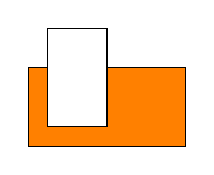
\begin{tikzpicture}
		\draw [fill=orange] (9,0) rectangle (11,1);
		\draw [fill=white] (9.25,0.25) rectangle (10,1.5);
		\end{tikzpicture}






	% ------------------------------------------ section ------------ 
	\newpage
	\section{선그리기}
	
	%	----------------------------------------------------
		\begin{tikzpicture}
		\draw [very thick] (0,0) to [out=90, in=195] (5,6.5);
		\end{tikzpicture}
		
		\begin{singlespace}
		\begin{verbatim}
		\begin{tikzpicture}
		    \draw [very thick] (0,0) to [out=90, in=195] (5,6.5);
		\end{tikzpicture}
		\end{verbatim}
		\end{singlespace}

	%	----------------------------------------------------
		\begin{tikzpicture}
		\draw [very thick] (0,0) to [out=45, in=180] (5,6.5);
		\end{tikzpicture}
	

		\begin{singlespace}
		\begin{verbatim}
		\begin{tikzpicture}
		\draw [very thick] (0,0) to [out=45, in=180] (5,6.5);
		\end{tikzpicture}
		\end{verbatim}
		\end{singlespace}

	%	----------------------------------------------------
		\begin{tikzpicture}
		\draw [very thick] 	
		    (0,0) to [out=0, in=0] 
		    (3,0) to [out=0, in=225] 
		    (5,1) to [out=45, in=225] 
		    (7,2) to [out=45, in=240] (10,6.5);
		\end{tikzpicture}

		\begin{singlespace}
		\begin{verbatim}
		\begin{tikzpicture}
		\draw [very thick] 	
		    (0,0) to [out=0, in=0] 
		    (3,0) to [out=0, in=225] 
		    (5,1) to [out=45, in=225] 
		    (7,2) to [out=45, in=240] (10,6.5);
		\end{tikzpicture}
		\end{verbatim}
		\end{singlespace}


	%	----------------------------------------------------
		
\begin{tikzpicture}
		\draw [very thick]
		    (0,0) to [out=90, in=180] 
		    (1,1) to [out=0, in=180] 
		    (2.5,0) to [out=0, in=225] (4,1);
		\end{tikzpicture}


		\begin{singlespace}
		\begin{verbatim}
		
\begin{tikzpicture}
		\draw [very thick]
		    (0,0) to [out=90, in=180] 
		    (1,1) to [out=0, in=180] 
		    (2.5,0) to [out=0, in=225] (4,1);
		\end{tikzpicture}
		\end{verbatim}
		\end{singlespace}




	% ------------------------------------------ section ------------ 
	\newpage
	\section{선그리기 : rounded corners }


		MANUAL Page 142
		
		\begin{tikzpicture}
		\draw [very thick]	 
					(0,0) 	[rounded corners=2cm] -- 
					(5,0) 	[rounded corners=2cm] -- 
					(7.5,5.0)[rounded corners=2cm] -- 
					(12,5.0) -- (15,0)	;
		\end{tikzpicture}



		\begin{singlespace}
		\begin{verbatim}
		\begin{tikzpicture}
		\draw [very thick]	 
		   (0,0) 	[rounded corners=2cm] -- 
		   (5,0) 	[rounded corners=2cm] -- 
		   (7.5,5.0)[rounded corners=2cm] -- 
		   (12,5.0) -- (15,0)	;
		\end{tikzpicture}
		\end{verbatim}
		\end{singlespace}



	% ------------------------------------------ section ------------ 
	\newpage
	\section{선그리기 : rounded corners의 응용예 }
	
	

























% ------------------------------------------------------------------------------
% End document
% ------------------------------------------------------------------------------
\end{document}


